\chapter{АНАЛИЗ ПРЕДМЕТНОЙ ОБЛАСТИ РЕКОМЕНДАТЕЛЬНЫХ СИСТЕМ}
\label{chap:analysis}
\aftertitle

\section{Понятие рекомендательных систем}

Задача фильтрации новостей и сообщений в групповых чатах решается рекомендательными системами. Рекомендательная система ~--  программная система, которая пытается предсказать, какие объекты (фильмы, музыка, книги, новости, веб-сайты) будут интересны пользователю, имея определенную информацию о его профиле \cite{recommendation_system_wiki}.

Существует несколько традиционных подходов к построению рекомендательных систем \cite{recommendation_system_methods}: контент-ориентированный подход и коллаборативная фильтрация.

Суть контент-ориентированного подхода заключается в сопоставлении атрибутов контента и пользователей. Например, здесь могут быть использованы категориальные атрибуты (жанр фильма, актеры фильма и т.п.), числовые атрибуты (продолжительность, рейтинг и т.п.) для составления эмбеддингов или вектора предмета ~-- векторных представлений объекта рекомендации. Аналогично составляется вектор пользователя. Построив эмбеддинги пользователя и объектов, можно осуществлять рекомендации. Объект рекомендуется пользователю, если его эмбеддинги близки к эмбеддингам пользователя, либо к эмбеддингам других объектов, купленных (просмотренных, прочитанных и т.п.) пользователем.

В качестве эмбеддингов могут выступать и различные текстовые описания. В классических рекомендательных системах могут использоваться такие методы, как TF-IDF \cite{no-patterns}, а в современных рекомендательных системах ~-- текстовые эмбеддинги, полученные с помощью больших языковых моделей \cite{tf_augumenting_recommendation}.

В последнее время активно развиваются подходы с использованием больших языковых моделей в рекомендательных системах.

\section{Развитие методов обработки естественного языка}

Большая языковая модель (Large Language Model, LLM) ~-- искусственная нейронная сеть, предназначенная для обработки и понимания естественного языка (natural language processing).

Языковые модели являются одним из способов решения задач обработки естественного языка и генерации текста. Языковые модели моделируют естественный язык путем генерации следующих или пропущенных слов в текстовых последовательностях. Развитие языковых моделей можно разделить на следующие этапы: статистические модели, базовые нейросетевые модели, предобученные модели и большие языковые модели \cite{llm_survey}. Эти этапы развития языковых моделей представлены на рисунке \ref{img:llm_evolution}.

\begin{figure}[h]
    \centering
    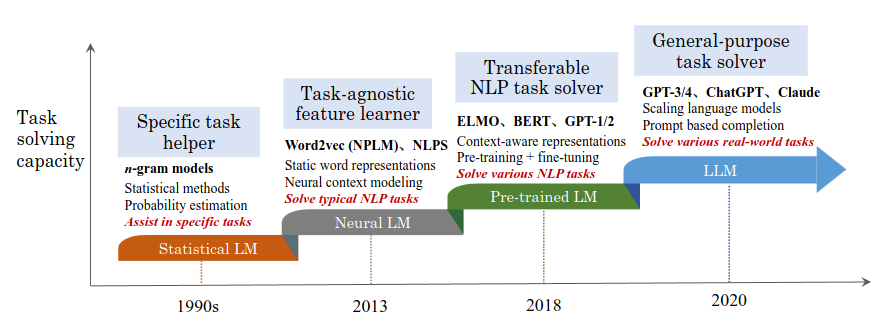
\includegraphics[width=\linewidth]{../images/llm_evolution.png}
    \caption{Развитие языковых моделей с точки зрения объема решаемых задач\cite{llm_survey}}
    \label{img:llm_evolution}
\end{figure}

Статистические модели основаны на классических методах машинного обучения и статистики. Типичным подходом к языковому моделированию являлось использованием марковских цепей для предсказания следующих элементов последовательности. Такие модели, имеющие фиксированный контекст из нескольких предыдущих элементов, называются n-gram моделями.

Следующим шагом в развитии языковых моделей стало использование искусственных нейронных сетей (сетей прямого распространения и рекуррентных нейронных сетей). Важным шагом стало создание векторных представлений слов (эмбеддингов), таких как word2vec \cite{word2vec}. Этот метод позволяет представлять слова текста в виде векторов, близость которых отражает семантическую близость слов. Подход word2vec основан на гипотезе локальности, которая утверждает, что слова, которые встречаются в одинаковых окружениях, имеют близкие значения. Этот и подобные методы продемонстрировали высокую эффективность в различных задачах обработки естественного языка. Подход с использованием нейронных сетей, в основном, рекуррентных нейронных сетей RNN и LSTM, позволил реализовать end-to-end модели, решающие различные типичные задачи обработки естественного языка.

Дальнейшим развитием этих принципов стали предобученные языковые модели. В отличие от word2vec, который обучается независимым от контекста представлениям, языковые модели способны понимать значение слова с учетом окружающего контекста.

Первой попыткой создания контекстуальных эмбеддингов стал Elmo \cite{elmo}. Эта модель способна запоминать представления слов, зависящие от контекста. Эта модель основана на архитектуре двусторонней LSTM.

Важным шагом в развитии моделей обработки естественного языка и в целом последовательностей стало появление архитектуры Трансформер \cite{transformer}. Трансформер представляет собой sequence-to-sequence модель, преобразующую текст (последовательность токенов) в другую последовательность токенов. Архитектурно он состоит из стека энкодеров, которые кодируют последовательность в некое внутреннее представление, и стека декодеров, которые генерируют новую последовательность. Важнейшим компонентом архитектуры Трансформера является механизм внимания (attention). Это механизм, который позволяет определять взаимную значимость токенов в последовательности, тем самым позволяя лучше выстраивать связи между токенами (словами), которые расположены далеко друг от друга. Ключевым вкладом архитектуры Трансформера был отказ от использования рекуррентных нейронных сетей и использование только лишь механизма внимания. Это позволило существенно улучшить вычислительную производительность модели и ее возможность к удержанию большого контекста, что, в свою очередь, дало возможность создавать большие модели, состоящие из десятков миллиардов параметров, что было бы невозможно с использованием рекуррентных нейронных сетей.

С тех пор архитектура Трансформер является основной архитектурой всех новейших state-of-the-art моделей по обработке естественного языка. На основе Трансформера были созданы такие получившие широкое распространение архитектуры, как BERT \cite{bert} и GPT \cite{gpt}.

Важной особенностью этих моделей является возможность использования трансферного обучения (transfer learning). Трансферное обучение ранее широко применялось в задачах компьютерного зрения. Суть данного метода заключается в использовании базовой модели, называемой backbone, которая обучена на большом количестве общих данных, которая затем дообучается на конкретных данных, специфичных для решаемой задачи. Это техника позволяет использовать очень глубокие нейронные сети, которые требуют большой объем обучающих данных и значительные вычислительные ресурсы для обучения.

Языковые модели обучаются с помощью техники self-supervised learning. Существуют различные методики обучения, такие как MLM (masked language modeling), CLM (casual language modeling) и др. В случае MLM некоторые слова (токены) в тексте заменяются на маску, задачей модели является предсказать закрытый токен. В случае CLM задачей модели является предсказать следующий токен последовательности. Это является ключевой частью успеха языковых моделей. Качество решения задач на естественном языке зависит от размера модели (количества параметров) и от объема обучающей выборки. Используемый подход позволяет обучать модели на очень больших объемах текстовой информации без необходимости в ручной разметке данных.

Обученная на большом корпусе текстов, языковая модель может выступать в качестве базовой модели для построения различных моделей для решения специфических задач, таких как определение тональности текста, фильтрация текста, чат-боты и рекомендательные системы.

Следующим шагом развития моделей обработки естественного языка стало появление больших языковых моделей. Было обнаружено, что с ростом размера модели (количества параметров) и объема обучающей выборки, результаты моделей улучшаются. Более того, большие модели показали качественно отличное поведение от моделей меньшего размера. C определенного размера модели происходит значительный нелинейный рост производительности моделей в различных задачах. Данное явление было названо эмерджентным поведением \cite{llm_emergent}. Зависимость метрик в различных задачах обработки естественного языка от количества параметров модели представлена на рисунке \ref{img:llm_scaling}.

\begin{figure}[h]
    \centering
    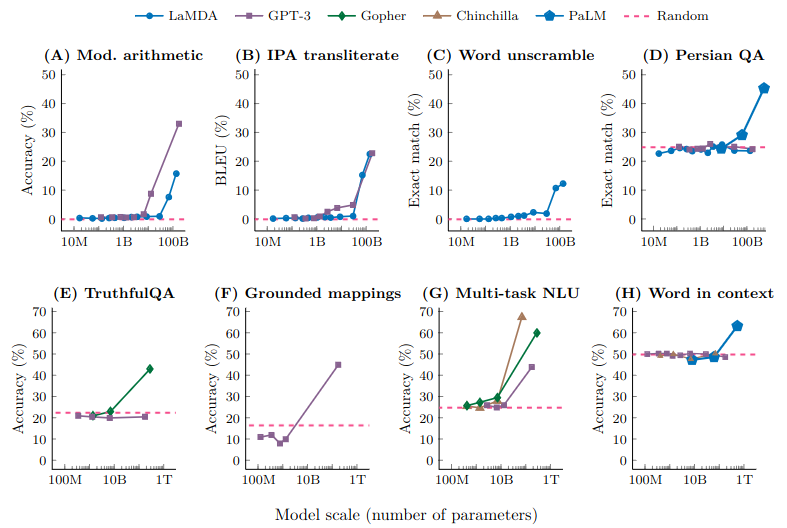
\includegraphics[width=\linewidth]{../images/llm_scaling.png}
    \caption{Зависимость метрик в различных задачах обработки естественного языка от количества параметров модели \cite{llm_emergent}}
    \label{img:llm_scaling}
\end{figure}

\section{Использование больших языковых моделей в рекомендательных системах}

Выдающиеся способности больших языковых моделей в задачах обработки естественного языка привлекли внимание многих исследователей, и в настоящее время тема применения больших языковых моделей в задачах построения рекомендательных систем активно исследуется \cite{do_llm_undertand_preferences, llm_rs_p5, llm_rs_survey}.

Большие языковые модели (LLM) обладают несколькими ключевыми преимуществами, которые делают их весьма эффективными в контексте рекомендательных систем.

Прежде всего, LLM проявляют высокий уровень понимания контекста, что делает их способными адаптироваться к сложным сценариям и улавливать тонкие нюансы в предоставленной информации. Это способствует повышению точности рекомендаций, учитывая текущий контекст и предпочтения пользователя.

Универсальность LLM проявляется в их способности решать различные рекомендательные задачи без необходимости создания отдельных алгоритмов для каждой из них. Это упрощает процесс интеграции модели в различные приложения и сценарии использования, снижая требования к инженерии.

LLM также эффективно справляются с проблемой холодного старта, обеспечивая качественные рекомендации, даже когда у пользователя ограниченный исторический след в системе. Это делает модели более устойчивыми и готовыми к предоставлению рекомендаций новым пользователям или тем, у кого ограниченный объем взаимодействий.

Преимущественное использование знаний, вложенных в модель, также выделяет LLM. Эти модели обладают обширными знаниями о мире, которые могут быть встроены в базовую модель, что снижает зависимость от конкретных обучающих датасетов. Это особенно полезно при обработке специфических сценариев, где требуются дополнительные знания.

Кроме того, LLM обеспечивают возможность объяснения принятых решений, что является важным аспектом для повышения доверия пользователей к рекомендациям. Модели могут предоставлять обоснование своих выводов, что помогает пользователям лучше понимать логику рекомендаций и повышает их удовлетворенность системой.

В работе \cite{llm_rs_survey} дается наиболее полный обзор существующих подходов к построению рекомендательных систем с использованием больших языковых моделей, а также приведена их классификация. Авторы разделяют все варианты использования больших языковых моделей в рекомендательных системах на две большие группы:
\begin{enumerate}
    \item discriminative models ~-- эти модели служат для генерации эмбеддингов, которые могут использоваться в существующих алгоритмах рекомендательных систем в качестве дополнительных данных;
    \item generative models ~-- эти модели обладают лучшей способностью к пониманию текста и используются в задачах генерации; при их использовании задача рекомендации преобразуется к задачам обработки естественного языка, в честности, с использованием text-to-text подхода.
\end{enumerate}

Можно выделить следующие парадигмы построения рекомендательных систем с использованием больших языковых моделей:
\begin{enumerate}
    \item преимущественно использование discriminative models:
          \begin{enumerate}
              \item LLM Embeddings + рекомендательная система ~-- при реализации данного подхода большая языковая модель используется в качестве средства извлечения признаков (feature extractor), генерирует эмбеддинги объектов, пользователей и их взаимодействия, которые затем используются алгоритмами рекомендательных систем;
          \end{enumerate}
    \item преимущественно использование generative models:
          \begin{enumerate}
              \item LLM Tokens + рекомендательная система ~-- данный подход похож на предыдущий, но выходом модели являются не эмбеддинги, а текст (последовательность токенов);
              \item LLM в качестве рекомендательной системы ~-- данный подход является end-to-end решением; на вход большой языковой модели подается запрос (промпт), содержащий описание задачи, описание пользователя, объектов и поведения пользователя; выходом модели являются рекомендации в той или иной форме.
          \end{enumerate}
\end{enumerate}

В свою очередь, при использования большой языковой модели непосредственно в качестве рекомендательной системы, возможны следующие варианты: рассуждение (reasoning), ранжирование (ranking) и предсказание следующей рекомендации.

Подход с использованием рассуждений основывается на общих знаниях больших языковых моделей (commonsense knowledge). При использовании данного подхода на вход большой языковой модели поступает запрос с описанием пользователя, взаимодействий пользователя и объектов, а также задание рекомендовать подходящие объекты. Выходом модели является текст с перечнем рекомендаций и объяснением. Преимуществом данного подхода является понятность, почему та или иная рекомендация была выбрана. Недостатком является ограниченность способности модели рекомендовать объекты только из того множества, которое известно на момент обучения и трудность к адаптации под существующие множество объектов (например, товаров в магазине).

Следующий подход ставит задачу рекомендации как задачу ранжирования, что близко к принципу действия традиционных рекомендательных систем. На вход модели поступает описание пользователя, возможно, другая информация, список предварительно отобранных объектов-кандидатов и задание проранжировать данные объекты. Возможны следующие стратегии ранжирования:
\begin{enumerate}
    \item pointwise ~-- модель предсказывает рейтинг каждого элемента независимо;
    \item pairwise ~-- модель выбирает предпочтительный объект из двух альтернатив;
    \item listwise ~-- модель ранжирует (сортирует) список объектов кандидатов.
\end{enumerate}

Классификация способов дообучения больших языковых моделей для использования в рекомендательных системах представлена на рисунке \ref{img:llm_rs_classification} \cite{llm_rs_survey}.

\begin{figure}[h]
    \centering
    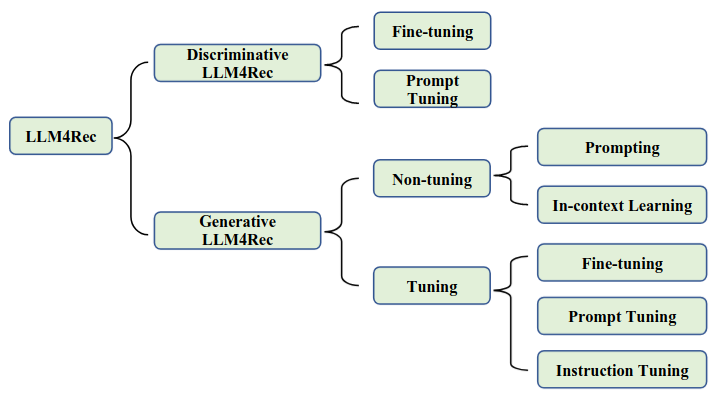
\includegraphics[width=\linewidth]{../images/llm_rs_classification.png}
    \caption{Способы дообучения больших языковых моделей для использования в задачах классификации \cite{llm_rs_survey}}.
    \label{img:llm_rs_classification}
\end{figure}

При использовании discriminative models существуют два способа дообучения моделей для решения специфических задач: с использованием классического дообучения (fine-tuning) и с помощью метода под названием prompt tuning \cite{llm_rs_survey}.

При дообучении предварительно обученная на большом корпусе текстов большая языковая модель, такая как BERT, дополнительно дообучается на сравнительно небольшом конкретном наборе данных для задачи. В процессе дообучения происходит обновление весов модели. При этом могут использоваться различные подходы к обучению, модель может дополняться слоями (например, слоем для классификации) и при обучении могут использоваться специальные для задачи функции ошибок. Дообучение большой языковой модели позволяет достичь лучших результатов при адаптации модели к выполнению задачи.

Тем не менее, дообучение модели имеет ряд недостатков. Для дообучения требуется большой объем данных. В связи с большим объемом данных и большой вычислительной сложностью модели (которая, зачастую, имеет от сотен миллионов до сотен миллиардов параметров), требуется большое время и значительные вычислительные ресурсы для дообучения. Кроме того, в процессе дообучения может произойти <<забывание>> моделью части имеющихся знаний \cite{prompt_tuning}.

Другим способом адаптации модели к решению конкретных задач является prompt engineering. В этом случае, модель не изменяется, но осуществляется подбор специального задания (промпта), который позволяет добиться лучшего результата. Такие сформированные человеком запросы называются hard prompt \cite{prompt_tuning}.

Другим способом адаптации модели к решению конкретных задач является prompt tuning. В этом случае осуществляется не ручной подбор запроса на естественном языке, а формирование эмбеддинга промпта с помощью механизма обратного распространения ошибки \cite{prompt_tuning}. Этот способ позволяет добиться результатов, близких к дообучению модели, но требует существенно меньших вычислительных ресурсов и меньшего объема обучающих данных.

При использовании генеративных моделей, существуют следующие способы адаптации моделей под задачу. Без обучения: prompting и in-context learning, и с обучением: дообучение (fine-tuning), prompt-tuning и instruction tuning.

Метод <<prompting>> использует возможности больших языковых моделей по выполнению задач, описанных на естественном языке, и заключается в подборке такого описания задачи (промпта), которые дает наилучшие результаты.

Метод <<in-context learning>> использует так называемый few-short learning. В этом случае небольшая обучающая выборка размером в несколько элементов, состоящая из пар <<значение-метка>> предоставляется модели непосредственно в запросе, в результате чего модель оказывается способна предсказывать метки для ранее неизвестных данных.

Дообучение (fine-tuning) при использовании генеративных моделей аналогично тому, как было описано ранее. Данный способ позволяет добиться лучших результатов, но требует значительных вычислительных ресурсов, потому что большие языковые модели, особенно, генеративные, такие как GPT-3, GPT-4, имеют очень большое количество параметров (от сотни миллиардов до триллиона параметров).

Метод <<prompt-tuning>> используется аналогично описанному ранее и позволяет достичь хороших результатов при меньших вычислительных затратах.

% Есть еще Instruction Tuning, но я пока что не поняла
% Думаю, обзор можно дополнить конкретными работами, не только этим обзорм, в которых приводятся примеры, как именно LLM работает с рекомендациями, какие там промпты итд

В работах \cite{news_rec_bert} и \cite{news_rec_gen} решается задача рекомендации новостей с использованием больших языковых моделей: в первой реализуется дискриминативный подход с использованием меньшей модели BERT, а во второй используется и дискриминативный подход с использованием большей модели LLaMA \cite{llama}, и генеративный подход с использованием ChatGPT \cite{chatgpt}. В обеих работах реализуется контентно-ориентированный подход.

Контентно-ориентированный подход формулируется следующим образом. Имеется множество $N$ объектов рекомендации (например, новостей), где каждый объект $n \in N$ представляется набором признаков: заголовком, описанием, категорией и т.п. Имеется множество пользователей $U$. И имеется множество предпочтений пользователя $D$. Каждый элемент $d \in D$ представлен кортежем $(u, n, y)$, который описывает, что пользователь $u$ выбрал ($y = 1$) или не выбрал ($y = 0$) объект $n$. Целью контентно-ориентированной рекомендательной системы является предсказание выбора пользователя на объекте-кандидате.

Контентно-ориентированная рекомендательная система состоит из трех основных элементов:
\begin{enumerate}
    \item энкодер контента (content encoder) ~-- генерирует представление контента в виде $d$-мерного вектора $v_n$;
    \item энкодер истории (history encoder) ~-- генерирует представление пользователя в виде $d$-мерного вектора $v_u$ на основе последовательности векторных представлений выбранных пользователем ранее объектов (например, прочитанных ранее новостей);
    \item модуль взаимодействия (interaction module или click-prediction module) ~-- определяет, выберет ли пользователь объект-кандидат на основе представлений $v_n$ и $v_u$, решая задачу бинарной классификации с классами: <<пользователь выберет>> и <<пользователь не выберет>>.
\end{enumerate}

В работе \cite{news_rec_bert} решается задача рекомендации новостей с использованием модели BERT. Архитектура решения представлена  на рисунке \ref{img:news_rec_bert}.

\begin{figure}[h]
    \centering
    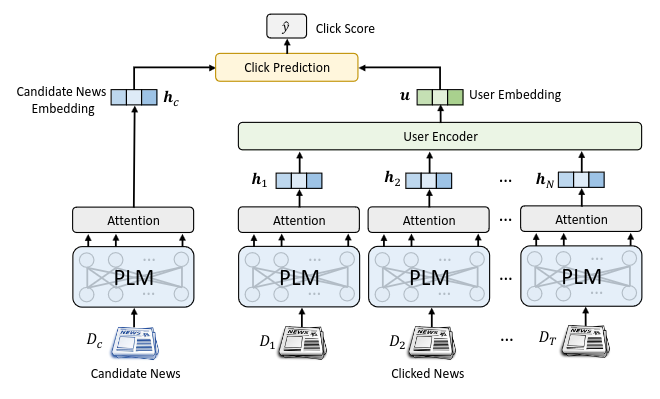
\includegraphics[width=\linewidth]{../images/news_rec_bert.png}
    \caption{Архитектура модели рекомендации новостей \cite{news_rec_bert}}.
    \label{img:news_rec_bert}
\end{figure}

Архитектура данного решения является типичной для контентно-ориентированных рекомендательных систем, которая была рассмотрена ранее. В данной работе BERT используется в качестве энкодера контента для новостей-кандидатов и новостей, просмотренных пользователем ранее, формируя эмбеддинги новостей $v_n$. Модель целиком дообучается на специальном датасете. В процессе обучения обучается как модуль взаимодействия (click prediction), так и дообучается модель BERT.

Задача рекомендации новостей с помощью больших языковых моделей также решается в работе \cite{news_rec_gen}. В этой работе используются сразу два подхода: открытые языковые модели (такие, как LLaMA) используются для извлечения признаков, закрытые языковые модели (такие, как ChatGPT) используются для преобразования и обогащения информации.

Система использует типичный для контент-ориентированных систем подход, аналогичный описанному ранее. Архитектура системы представлена на рисунке \ref{img:news_rec_gen} и состоит из модуля энкодера контента, модуля энкодера пользователя и модуля взаимодействия.

\begin{figure}[h]
    \centering
    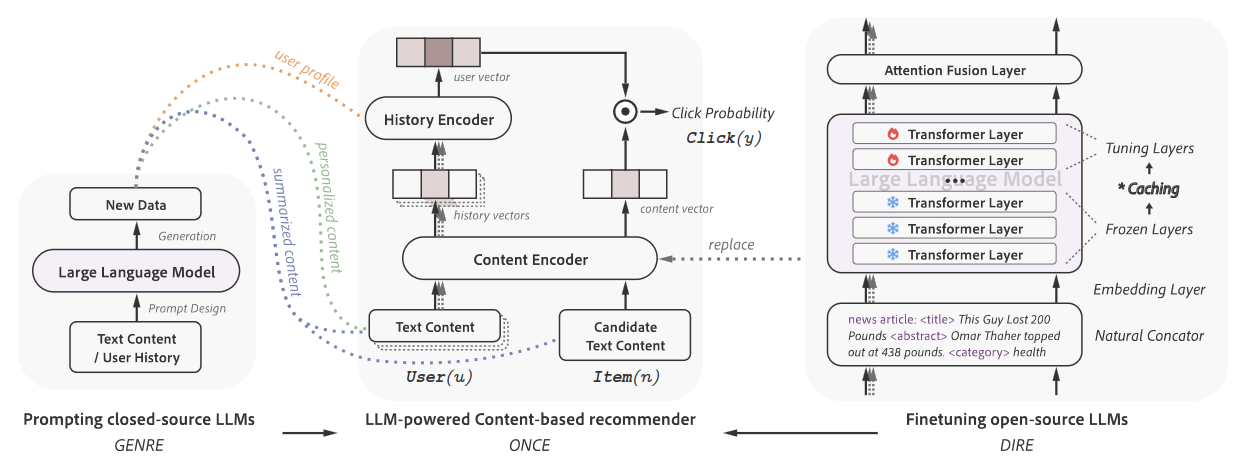
\includegraphics[width=\linewidth]{../images/news_rec_gen.png}
    \caption{Архитектура модели рекомендации новостей \cite{news_rec_gen}}.
    \label{img:news_rec_gen}
\end{figure}

В ряде исследований использовались большие языковые модели непосредственно для генерации рекомендаций без дообучения с использованием промптинга и техники in context learning. Тем не менее, такие подходы уступают классическим методам рекомендательных систем с использованием коллаборативной фильтрации. Поэтому, в данной работе большая языковая модель не используется непосредственно для генерации рекомендаций.

Закрытая большая языковая модель GPT-3.5 используется для предварительной обработки данных перед их передачей в энкодер. Предварительная обработка позволяет получить дополнительные признаки, которые улучшают работу рекомендательной системы. В работе применяются следующие методы предобработки:
\begin{enumerate}
    \item суммаризация контента ~-- LLM используется для суммаризации заголовка, описания и текста новости и получение нового более информативного описания новости;
    \item формирование профиля пользователя ~-- LLM используется для определения тем интереса и регионов интереса пользователя на основе истории просмотренных ранее новостей;
    \item генерация синтетического персонализированного контента ~-- LLM используется для генерации рекомендаций на основе профиля пользователя и его истории просмотренных новостей. Разумеется, LLM дает рекомендации тех объектов, которые известны ей из обучающей выборки и не способна рекомендовать реальные объекты, с которыми работает система. Тем не менее, такой подход позволяет обогатить данные, особенно для новых пользователей с маленькой историей просмотров.
\end{enumerate}

Энкодер контента, который конвертирует текстовое описание пользователя, истории и новостей в векторное представление, основан на открытой большой языковой модели LLaMA. Модель дополнена слоями: линейный слой используется для уменьшения размерности внутренних представлений, слой внимания используется для объединения последовательности скрытых состояний в один вектор.

В отличие от работ, которые используют модели меньшего размера и применяют специальные токены для разделения различных признаков объекта (таких как заголовок, описание и т.п.), в этой работе формируют текстовое представление объекта на естественном языке, например, <<news article: <title> ..., <category> ..., <abstract> ...>>.

Для уменьшения времени и вычислительных ресурсов, требующихся для дообучения большой языковой модели, используются следующие техники. Во-первых, большая часть слоев модели <<замораживается>>, т.е. их веса не обучаются в процессе обучения, а обучаются только несколько последних слоев. Также, внутреннее представление <<замороженных>> слоев рассчитывается однократно для каждого элемента из датасета и кэшируется. Таким образом, при нескольких эпохах обучения не требуется повторно вычислять значения замороженных слоев, которые, очевидно, не изменяются в процессе обучения. Во-вторых, применяется техника под названием Low-Rank Adaptation (LoRA) \cite{lora}, которая позволяет существенно уменьшить количество обучаемых параметров и, следовательно, уменьшить необходимые вычислительные ресурсы.

\section{Обзор аналогов}

Задача рекомендации новостей широко используется. Фактически, рекомендательные системы встроены практически в каждый крупный агрегатор новостей, веб-сайты новостных и информационных агенств, социальные сети, блог-платформы и т.п.

Например, веб-сайт информационного агентства <<РИА Новости>> \cite{ria_news} содержит блок рекомендации похожих новостей на странице новости. Тем не менее, сайт не имеет возможности показа персонализированных подборок новостей и их суммаризации.

Другим примером является является блог-платформа и новостной агрегатор <<Дзен>> \cite{dzen}. Основой этого ресурса является лента новостей и блог-постов, которая подстраивается под интересы пользователя. Данный ресурс не имеет возможности предоставлять суммаризации новостей.

Telegram \cite{telegram} является популярным мессенджером и новостной платформой в ряде стран. Наиболее популярен в России, Украине, Индии и Иране. В России в 2023 году охват пользователей составил 45.8\% населения и занимает седьмое место в рейтинге самых популярных интернет-площадок. Telegram является восьмой по популярности социальной сетью в мире и имеет 800 миллионов пользователей. Чаще всего пользователи регулярно читают 6-10 каналов \cite{telegram_stat}.

Таким образом, Telegram является популярным ресурсом с большой аудиторией. Все больше пользователей предпочитают читать новости в Telegram и использует его как основной источник новостей. Тем не менее, практически не представлено рекомендательных систем, предоставляющих рекомендации новостей в Telegram.

В работе \cite{tg_rs_1} рассматривается построение рекомендательной системы каналов для Telegram. В работе автор использовал сообщения пользователей в групповом чате и использовал их для персональных рекомендаций каналов. Для генерации векторных представлений использовался метод TF-IDF. Данная работа не решает поставленных целей: система осуществляет рекомендации каналов, а не отдельных новостей, и работает только для пользователей определенного чата, следовательно, не может быть использована произвольным пользователем. Также существует проблема холодного старта ~-- без набора значительного количества сообщений от пользователя, система не сможет выдавать корректные рекомендации. Кроме того, эмбеддинги на основе TF-IDF существенно уступают современным языковым моделям.

Аналогично решается задача рекомендации пользователям каналов в Telegram в работе \cite{tg_rs_2}. Используется TF-IDF для формирования эмбеддингов пользователей и групп. Для оптимизации производительности при работе с большим количеством пользователей и каналов используется кластеризация. Данная работа имеет аналогичные недостатки: система осуществляет рекомендации каналов, а не отдельных новостей, использует TF-IDF.

В еще одной работе \cite{tg_rs_3} реализуется система рекомендации каналов в Telegram. В отличие от двух предыдущих работ, которые основаны на контентно-ориентированном подходе, в этой работе используется коллаборативная фильтрация. Решение, представленное в этой работе, имеет аналогичные недостатки.

Таким образом, в результате анализа аналогов, не было обнаружено существующих решений, которые могут осуществлять персонализированные рекомендации новостей в Telegram, и, тем более, предоставлять суммаризированную сводку из новостных каналов и публичных чатов.
